%************************************************
\chapter{Distillation (Introduction)}
%************************************************
\begin{flushright}
February 26, 2013
\end{flushright}
\section{Aim}
To purify Ethyl Acetate using the distillation technique.

\section {Chemicals Required}
	\begin{enumerate}
		\item Ethyl Acetate
	\end{enumerate}

	% \begin{figure}[bth]
	% 	\begin{center}
	% 		
\includegraphics[width=0.2\linewidth]{gfx/e5_compound1}
	% 	\end{center}
	% \caption[Aniline]{\label{e5_compound1}}
	% \end{figure}

	% \begin{figure}[bth]
	% 	\begin{center}
	% 		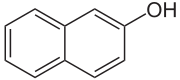
\includegraphics[width=0.4\linewidth]{gfx/e5_compound2}
	% 	\end{center}
	% \caption[2-Naphthol]{\label{e5_compound2}}
	% \end{figure}
\section {Apparatus/Setup}
	\begin{figure}[bth]
		\begin{center}
			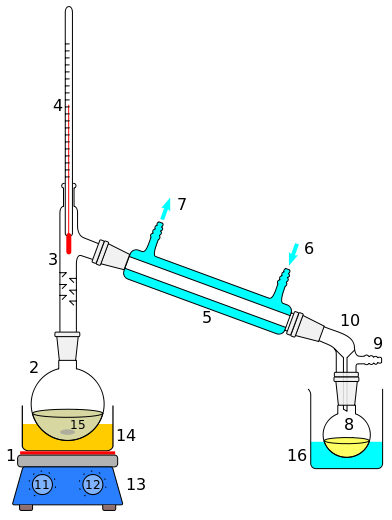
\includegraphics[width=0.7\linewidth]{gfx/e6_setup}
		\end{center}
	\caption[Distillation Setup]{\label{e6_setup}}
	\end{figure}
	Refer to \autoref{e6_setup} for a schematic of the setup and the following for a description. The image was taken from Wikipedia.
	\begin{enumerate}
		\item Heating Device
		\item Still Pot
		\item Still Head
		\item Thermometer
		\item Condenser
		\item Cooling water input		
		\item Cooling water output [if the nozzels are in opposite directions, this is the one which is higher, to ensure the water's completely filled in the condenser]
		\item Disillate/receiving flask
		\item Vaccuum/gas inlet [we didn't use this]
		\item Still receiver
		\item Heat control
		\item Stirrer speed control [we didn't use a stirrer]
		\item Stirrer/heat plate [we didn't have this in our setup]
		\item Heating (Oil/Sand) bath [we used an electric heater instead]
		\item Stirring Mechanism (heating beads were used)
		\item Cooling Bath (this wasn't used)
	\end{enumerate}


\section{Theory}
	Distillation as described in wikipedia is a method of separating mixtures based on the differences in the volatility of its constituents.
	\par
	The idea is rather simple. To make it easy to follow, please refer to \autoref{e6_setup} and understand the labels. The mixture is heated. The constituent with a lower boiling point would initiate boiling at a lower temperature, which is maintained by adjusting the heater and using the thermometer. The vapours of this constituent pass through the condenser and condense. Then gravity pushes these vapours from the condenser to the receiving flask. Temperature of the vapour helps determine which constituent is being collected.
	\par
	For this experiment however, we didn't use a mixture. Instead we used Ethyl Acetate and distilled that to purify it.

\section{Procedure}	
	\begin{enumerate}
		\item The system was setup as shown in \autoref{e6_setup}
		\item The water circulator was turned on after submersing it in a large water bath
		\item The heating was initiated and temperature monitored to keep it in the 75 - 80 $^o C$ range
		\item When most of the content had been transferred, the process was stopped. (Some liquid was left in the flask to avoid adverse effects)
	\end{enumerate}
	% \begin{enumerate}
	% 	\item Initial Setup
	% 		\begin{enumerate}
	% 			\item TLC plates were prepared
	% 			\item The visibility chamber was prepared
	% 			\item TLC was run at a suitable concentration of Ethyl Acetate, with the mixture and both compounds as given in the figure.
	% 		\end{enumerate}
	% 	\item Method 1: Using $NaHCO_3$ first
	% 		\begin{enumerate}
	% 			\item The given mixture was taken in a separating funnel (after ensuring it's clean of course)
	% 			\item To the mixture $NaHCO_3$ was added and the funnel shaken well
	% 			\item The two layers were allowed to separate
	% 			\item The bottom layer was extracted in a beaker
	% 			\item Again $NaHCO_3$ was added and the procedure repeated
	% 			\item The organic layer should now contain only Aniline; This was confirmed by running a TLC
	% 			\item The contents of the beaker were neutralized using a pH paper and $HCl$
	% 			\item The content of the beaker was transferred into the separating funnel again and Ethyl Acetate was added, shaken
	% 			\item Both layers were collected in separate beakers and the aqueous layer was again put into the separating funnel, and the process repeated
	% 			\item The organic layer extracted should contain only Naphthol; This was confirmed by running a TLC
	% 		\end{enumerate}
	% 	\item Method 2: Using $HCl$ first\\			
	% 		The process is identical to the previous case, except for the role of $HCl$ and $NaHCO_3$ which were swapped systematically
	% \end{enumerate}

\section{Observations and Results}
	The evaporation seemed to have started at $44-45 ^o C$, however the temperature was found to have stabilized at $77 ^o C$. Most of the Ethyl Acetate was evaporated and collected in the receiving flask successfully.

\section{Precaution}
	\begin{enumerate}
		\item Do not forget to use boiling chips, else unequal heat spread may result in explosive circumstances
		\item The water output should be facing upwards
		\item The condenser tube should be sufficiently slanted in the right direction to ensure the condensed liquid flows to the receiving flask and not the other way.
	\end{enumerate}

	
\section{Acknowledgements}
I thank Dr. R Vijaya Anand for his guidance during the experiment. I also acknowledge the contribution of my lab partners, Vivek, Prashansa and Srijit for performance of the same. I also thank our PhD guide for demonstrating the experiment and her assistance in general, with performance of the same.

	% \clearpage
	% \begin{figure}[bth]
	% 	\begin{center}
	% 		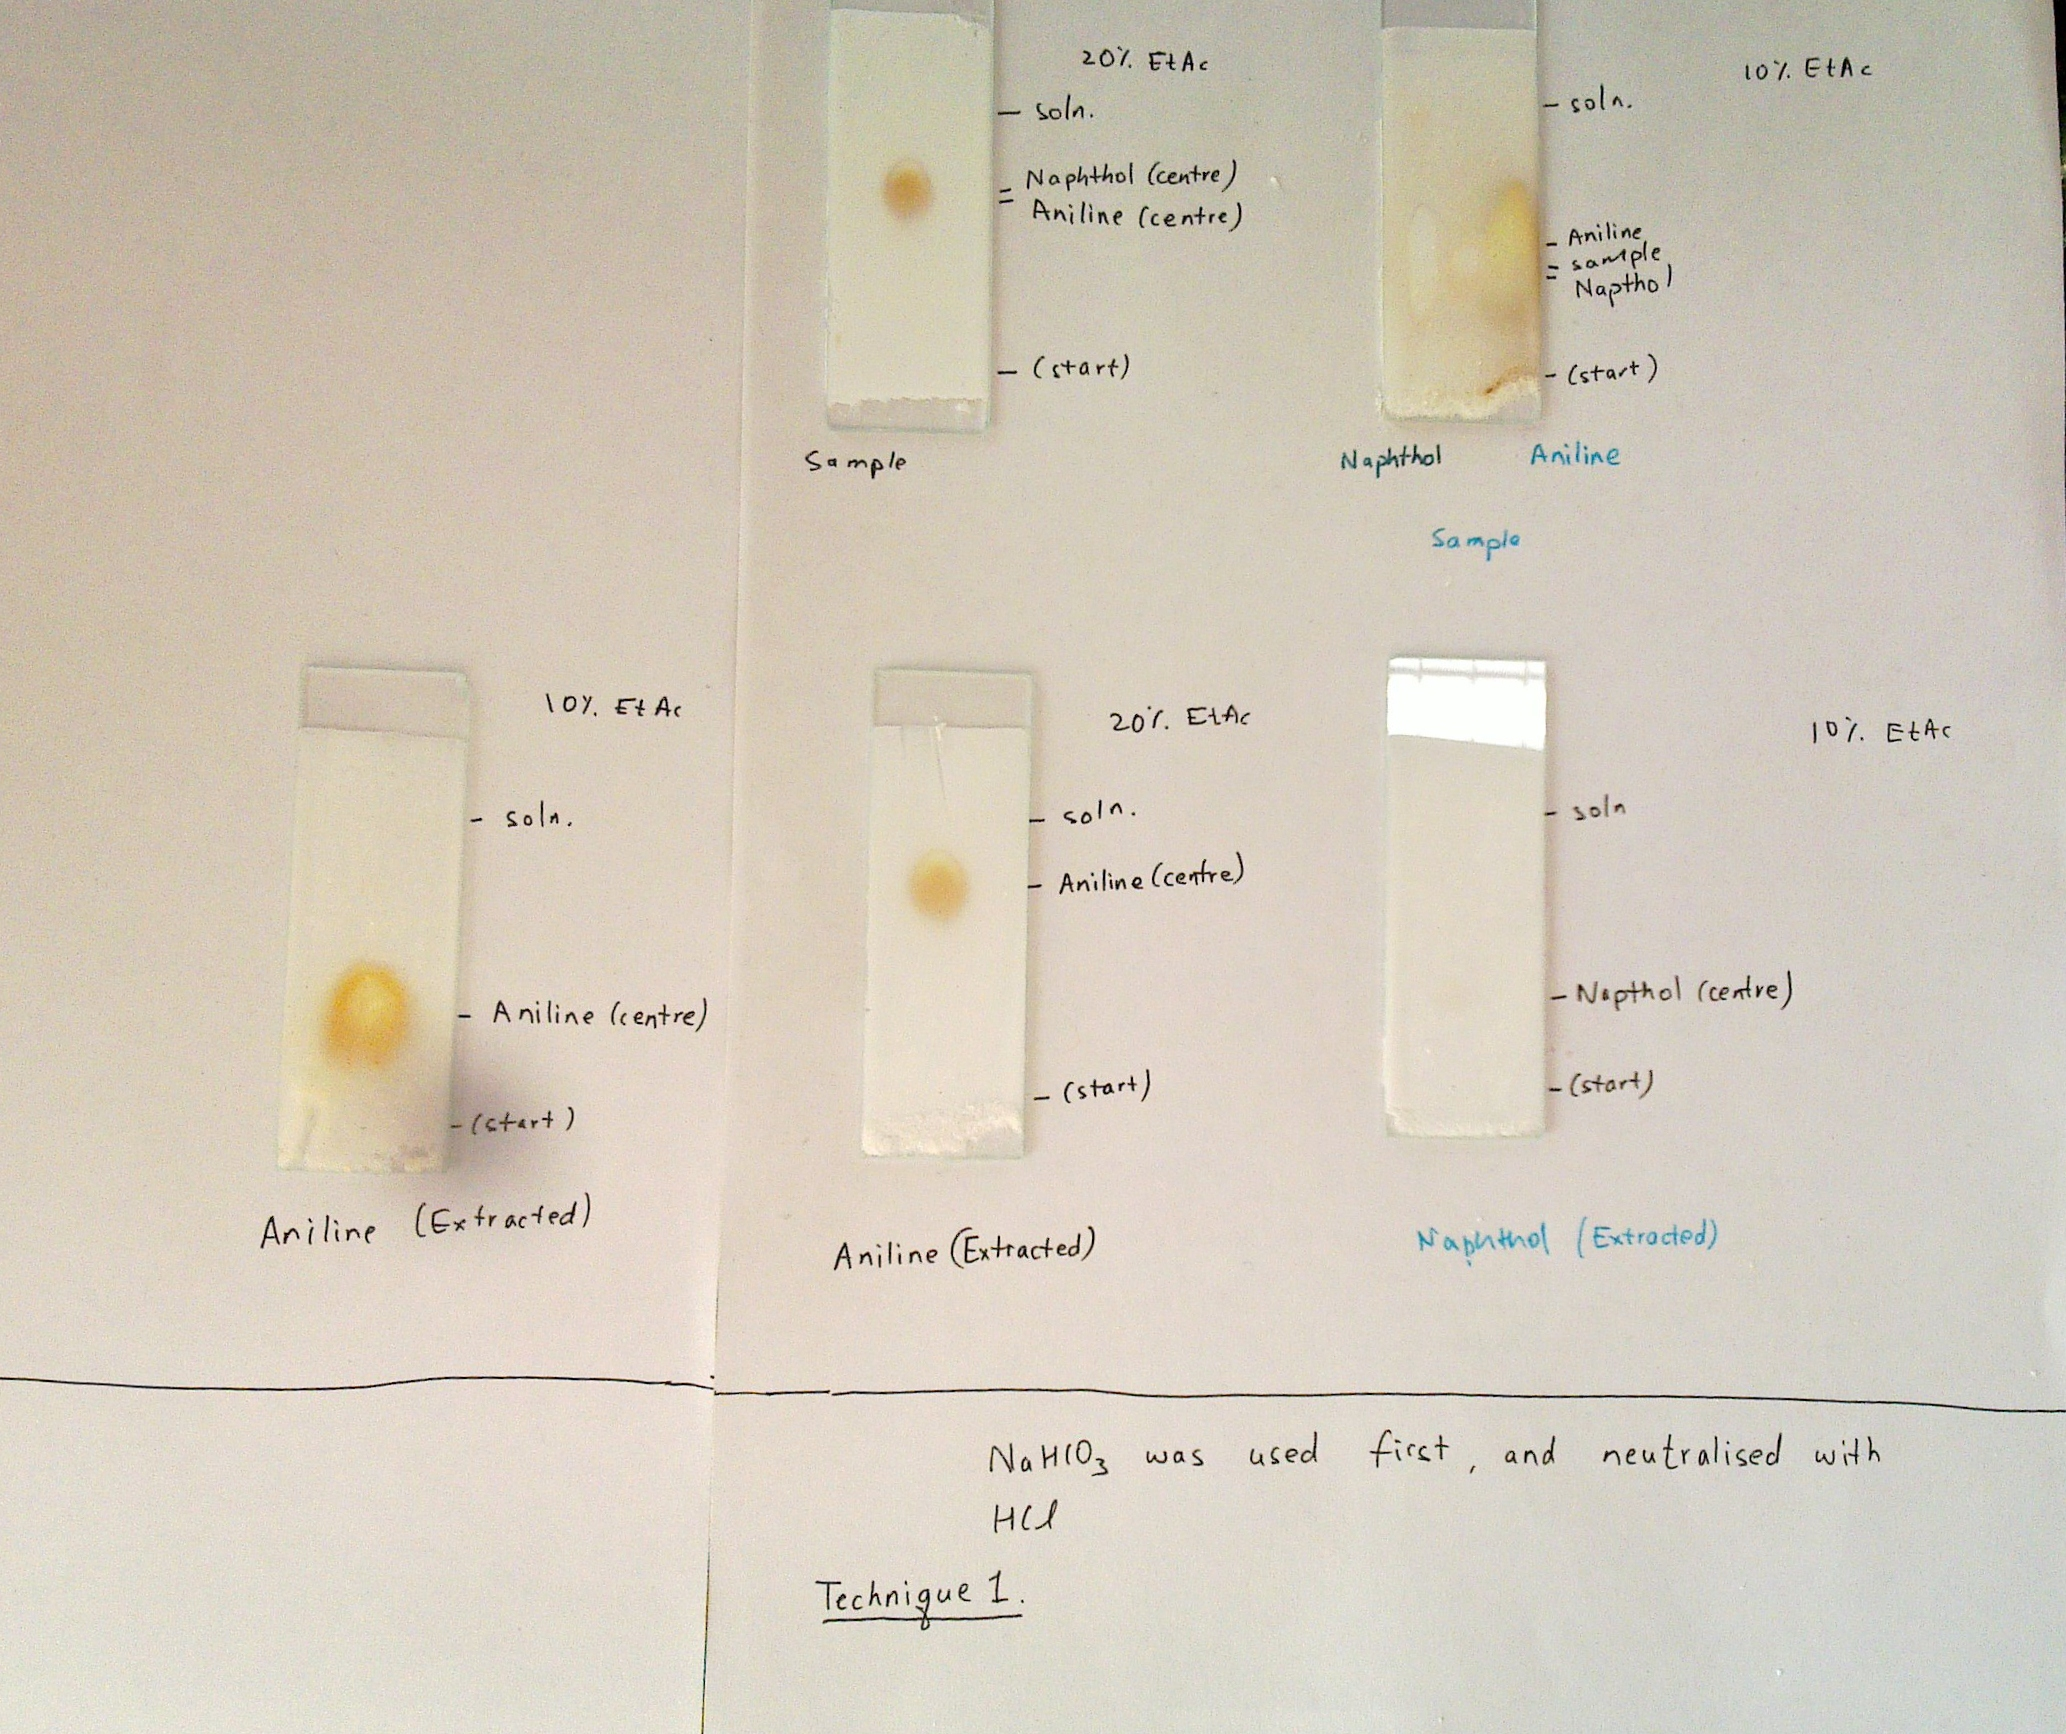
\includegraphics[width=1.5\linewidth]{gfx/e5_1}
	% 	\end{center}
	% \caption[TLCs Set 1]{\label{e5_1}}
	% \end{figure}

	% \begin{figure}[bth]
	% 	\begin{center}
	% 		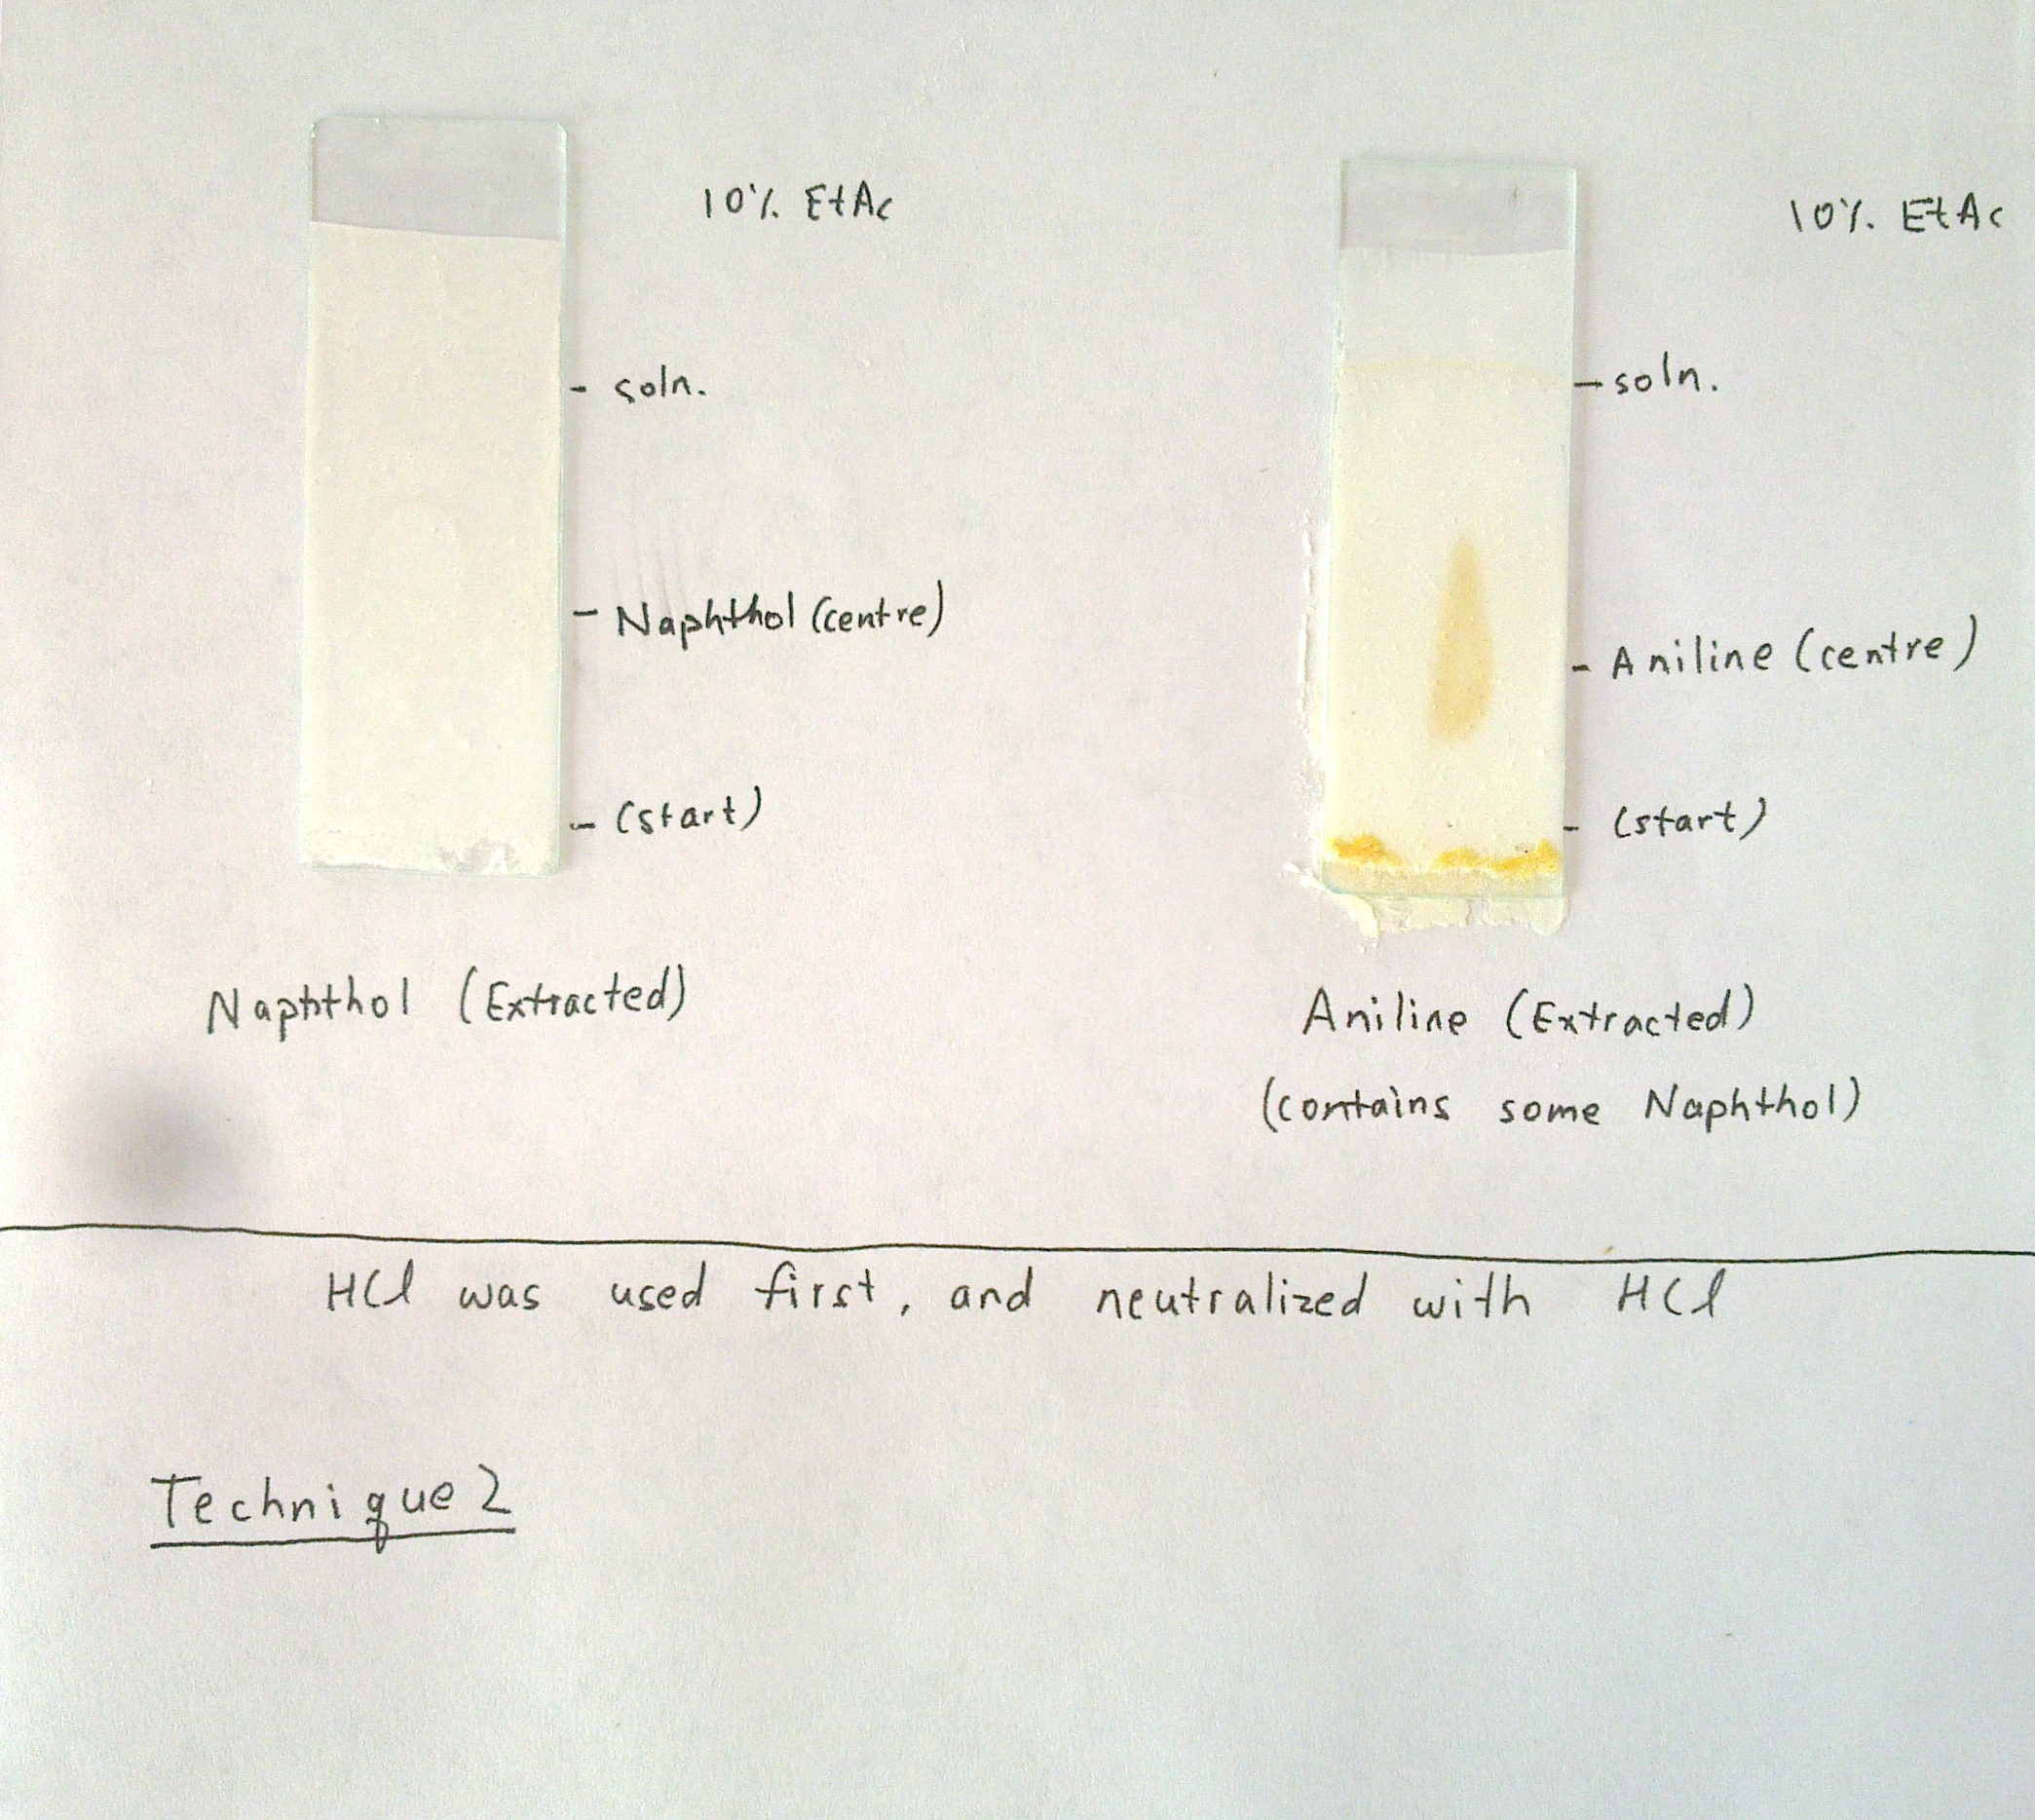
\includegraphics[width=1.0\linewidth]{gfx/e5_2}
	% 	\end{center}
	% \caption[TLCs Set 2]{\label{e5_2}}
	% \end{figure}